
\begin{exercise}{Fourier-Analyse }
\label{ex-de-mt-fourier-2}
\begin{itemize}
  \item Erkl�ren Sie kurz und ohne Formeln die Grundlagen und Funktionsweise von Fourierreihen (Fourierkoeffizienten und deren Bedeutung)
  \item Fourierreihen lassen sich eigentlich nur bei periodischen Signalen nutzen. Wie kann man diese Einschr�nkung umgehen und auch nichtperiodische Signale damit beschreiben?
  \item Skizzieren sie f�r eine reine Sinuskurve mit einer Frequenz von 1000Hz das Originalsignal sowie den Frequenzraum.
  \item Skizzieren sie den Frequenzraum f�r folgendes Signal: $f(x)=sin(8\pi x)+sin(2\pi x)+sin(200\pi x)$
  \item Ordnen sie die unten angef�hrten Signalverl�ufe (a-c) den entsprechenden Frequenzspektren (1-3) zu.\\[2ex]
  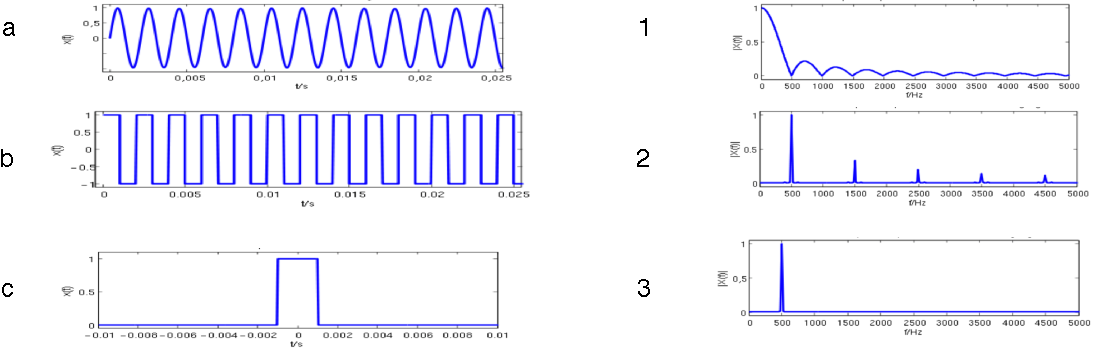
\includegraphics[width=0.8\textwidth]{figure/spektren}
\end{itemize} 
\end{exercise}